\chapter{Исследовательская часть}

\section{Технические характеристики}
Технические характеристики устройства, на котором выполнялись замеры по времени, представлены далее.
\begin{itemize}
	\item Процессор: AMD Ryzen 5 5500U\,--\,2.10 ГГц;
	\item Оперативная память: 16 ГБайт;
	\item Операционная система: Windows 10 Pro 64-разрядная система версии 22H2.
\end{itemize}

При замерах времени ноутбук был включен в сеть электропитания и был нагружен только системными приложениями.

\section{Демонстрация работы программы}
На рисунке \ref{img:demonstration} представлена демонстрация работы разработанного ПО.  
\begin{figure}[h]
	\centering
	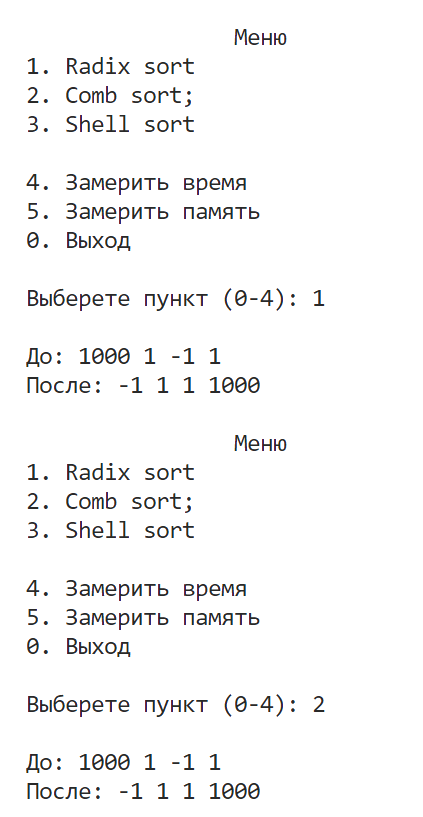
\includegraphics[height=0.3\textheight]{img/prog_work.png}
	\caption{Демонстрация работы программы}
	\label{img:demonstration}
\end{figure}

\section{Затраты по времени выполнения реализаций алгоритмов}
Все замеры проводились на квадратных матрицах. Поскольку замеры по времени имеют некоторую погрешность, замеры производились 100 раз, а затем вычислялось среднее арифметическое значение.

Результаты замеров приведены в таблицах \ref{tbl:time_even}--\ref{tbl:time_odd}.

На рисунках \ref{plt:time_01}--\ref{plt:time_03} приведены графики зависимостей работы алгоритмов от размеров матриц.

\begin{table}[h!]
    \caption{Результаты замеров времени (четные размеры матрицы)}
    \label{tbl:time_even}
	\centering
		\begin{tabular}{||c|c|c|c||}
			\hline
			& \multicolumn{3}{c|}{Время, мкс} \\ \cline{2-4}
			Размер матрицы & Стандартный & Виноград & (опт.) Виноград
			\csvreader{tables/time_even.csv}{}
			{\\\hline \csvcoli & \csvcolii & \csvcoliii & \csvcoliv} 
			\\
			\hline
		\end{tabular}
\end{table}

\begin{table}[h!]
    \caption{Результаты замеров времени (нечетные размеры матрицы)}
    \label{tbl:time_odd}
	\centering
		\begin{tabular}{||c|c|c|c||}
			\hline
			& \multicolumn{3}{c|}{Время, мкс} \\ \cline{2-4}
			Размер матрицы & Стандартный & Виноград & (опт.) Виноград
			\csvreader{tables/time_odd.csv}{}
			{\\\hline \csvcoli & \csvcolii & \csvcoliii & \csvcoliv} 
			\\
			\hline
		\end{tabular}
\end{table}

\begin{table}[h!]
    \caption{Результаты замеров времени (размер матрицы~--- степень двойки)}
    \label{tbl:time_ext}
	\centering
		\begin{tabular}{||c|c|c|c|c||}
			\hline
			& \multicolumn{4}{c|}{Время, мкс} \\ \cline{2-5}
			Размер матрицы & Стандартный & Виноград & (опт.) Виноград & Штрассен
			\csvreader{tables/time_ext.csv}{}
			{\\\hline \csvcoli & \csvcolii & \csvcoliii & \csvcoliv & \csvcolv} 
			\\
			\hline
		\end{tabular}
\end{table}

\clearpage

\begin{figure}[H]
	\centering
	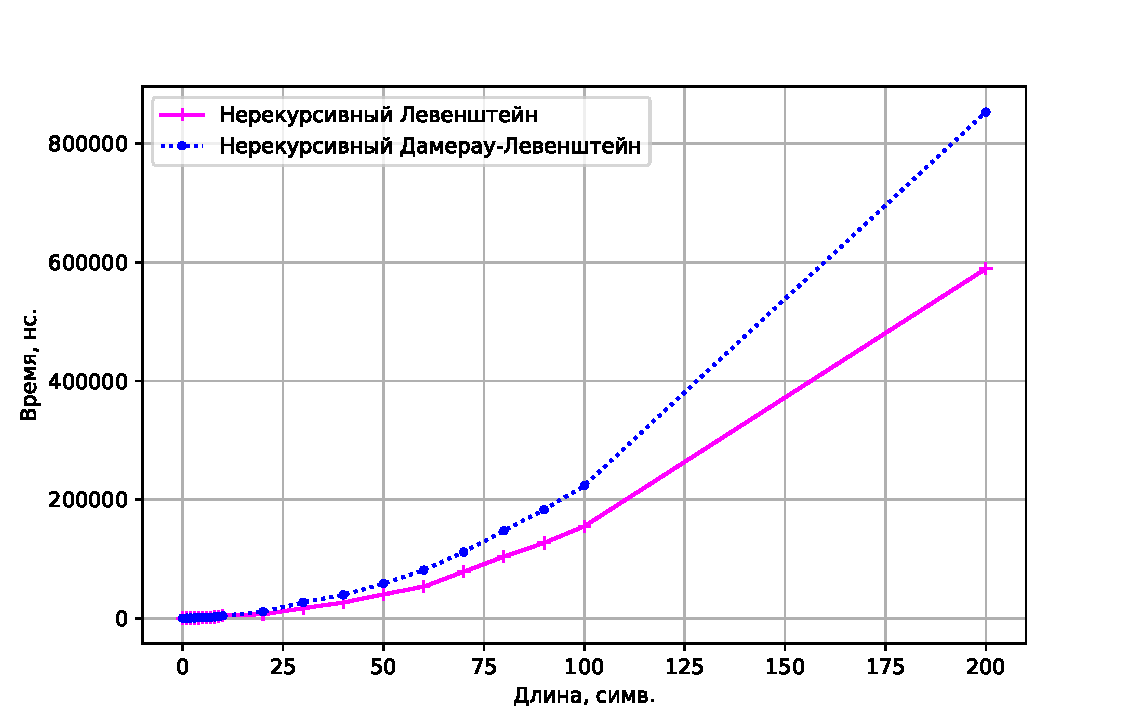
\includegraphics[height=0.4\textheight, page=1]{img/figures.pdf}
	\caption{Сравнение по времени алгоритмов умножения матриц на четных размерах матрицы}
	\label{plt:time_01}
\end{figure}


\begin{figure}[H]
	\centering
	\includegraphics[height=0.4\textheight, page=2]{img/figures.pdf}
	\caption{Сравнение по времени алгоритмов умножения матриц на нечетных размерах матрицы}
	\label{plt:time_02}
\end{figure}

\clearpage

\begin{figure}[H]
	\centering
	\includegraphics[height=0.4\textheight, page=3]{img/figures.pdf}
	\caption{Сравнение по времени алгоритмов умножения матриц на размерах, равных степени двойки}
	\label{plt:time_03}
\end{figure}

\section{Затраты по памяти реализаций алгоритмов}

\section*{Вывод}
